\documentclass[11pt]{article}
\pdfoutput=1

\usepackage[T1]{fontenc}
\usepackage[utf8]{inputenc}
\usepackage[brazil]{babel} 
\usepackage{import}
\usepackage[toc,page]{appendix}
\usepackage{latexsym,amsfonts,amsmath,amssymb,mathrsfs,bbold,mathtools,esint,amsthm,mathtools,mathptmx}
\usepackage{dsfont}
\usepackage{mathtools}
\usepackage{float}
\usepackage{graphicx}
\usepackage{cite}
\usepackage{hyperref}
\usepackage{setspace}
\usepackage{color}
\usepackage{slashed}
\usepackage{cleveref}
\numberwithin{equation}{section}
\usepackage[colorinlistoftodos]{todonotes}
\usepackage[affil-it]{authblk}
\renewcommand\Authand{ e } 
\usepackage{float}
\usepackage{indentfirst}
\usepackage{soul}
\usepackage{booktabs}
\usepackage{eso-pic,graphicx}
\usepackage{nicefrac}
\usepackage{epsfig}
\usepackage[a4paper]{geometry}
\usepackage{makeidx}
\usepackage{fancyhdr}

\graphicspath{{/images}}

%--- PAGE LAYOUT >> PARA a4 COM ONESIDE ---
\usepackage{a4wide}
\topmargin 0in
%--- PAGE STYLE >> PARA a4 COM ONESIDE ---
  \pagestyle{fancy}                            
  \renewcommand{\sectionmark}[1]{%             %
    \markright{\thesection\ #1}}               %
  \fancyhf{}                                   % - limpar configurações
  \fancyhead[LE,RO]{\bfseries\thepage}         % - externo - número da página
  \fancyhead[LO]{\bfseries\nouppercase{\rightmark}}% - interno ímpar - seção
  \fancyhead[RE]{\bfseries\nouppercase{\leftmark}}% - interno par - capítulo
  \renewcommand{\headrulewidth}{0.5pt}         % - linha horizontal
  \renewcommand{\footrulewidth}{0pt}           %
  \addtolength{\headheight}{0.5pt}             % - espaço para a linha
  \fancypagestyle{plain}{%                     %
    \fancyhead{}                               % - sem cabeçalhos em páginas limpas
    \renewcommand{\headrulewidth}{0pt}         % - sem linhas
  }

\setcounter{MaxMatrixCols}{10}

\usepackage{color,hyperref}
\definecolor{darkblue}{rgb}{0.0,0.0,0.3}
\hypersetup{colorlinks,breaklinks,
            linkcolor=darkblue,urlcolor=darkblue,
            anchorcolor=darkblue,citecolor=darkblue}

\usepackage{palatino}

%%%%%% Comece a editar o arquivo a partir desta linha %%%%%%

\title{Características eletrônicas, síntese e aplicações de pontos quânticos}
\author[1]{Alan Abdalad Vianna\footnote{\href{mailto:alan@alunos.eel.usp.br}{alan@alunos.eel.usp.br}}}
\author[1]{Ângelo Augusto Santos Marcolin\footnote{\href{mailto:angelo.marcolin@usp.br}{angelo.marcolin@usp.br}} }
\author[1]{Bruno Sardinha Alves Pereira\footnote{\href{mailto:bruno.sap@alunos.eel.usp.br}{bruno.sap@alunos.eel.usp.br}} }
\author[1]{Caroline Teixeiera Lisboa\footnote{\href{mailto:caroline.tl@alunos.eel.usp.br}{caroline.tl@alunos.eel.usp.br}} }
\author[1]{Vitor Gabriel Fernandes\footnote{\href{mailto:vitor.gf@alunos.eel.usp.br}{vitor.gf@alunos.eel.usp.br}} }
\author[1]{Vinícius Rodrigues Costa\footnote{\href{mailto:vinicius.rc@alunos.eel.usp.br}{vinicius.rc@alunos.eel.usp.br}} }
\author[1]{Yasmin Michelin dos Santos\footnote{\href{mailto:yasmin.michelin@usp.br}{yasmin.michelin@usp.br}} }

\affil[1]{Escola de Engenharia de Lorena\\
Universidade de São Paulo\\
12602-810, Lorena, SP, Brasil}


\begin{document}
\onehalfspacing

\maketitle

\abstract{Introduza um resumo aqui.}

\tableofcontents

\section{Introdução}


\par De acordo com André Rezende\cite{introducao1}, pontos quânticos são nanopartículas semicondutoras, que por terem o tamanho reduzido, se comportam como um poço de potencial. Isso faz com que elétrons e buracos sofram um forte confinamento quântico nas três dimensões espaciais. Devido a esse confinamento, eles têm sua energia quantizada em valores discretos, como em um átomo, por isso também são chamados de átomos artificiais.

\par A história dessas nanopartículas começa em 1980 em um artigo publicado pelo físico russo, Ekimov. Seu trabalho foi baseado no estudo de efeitos quânticos de tamanho em cristais semicondutores microscópicos em três dimensões. Segundo Ekimov \cite{introducao2}:

\begin{quote}
\textit{"Apresentamos a descoberta e a espectroscopia de uma nova classe de objetos que exibem efeitos quânticos de tamanho: cristais microscópicos tridimensionais de compostos semicondutores crescidos em uma matriz dielétrica transparente."}
\end{quote}

\par Apesar de tratar como uma nova classe de objetos, Ekimov não os denomida nem os trata como pontos quânticos.

\par Durante seu estudo, ao realizar a absorção espectral de três amostras de cristais microscópicos com raios diferentes, observou uma dependência na posição espectral das linhas de absorção, onde supôs se tratar de um efeito quântico de tamanho ocorrido devido ao tamanho da partícula, e complementa:

\begin{quote}
\textit{“Tais portadores de carga na matriz dielétrica estão presos em um poço de potencial onde as paredes são limitadas pelo cristal microscópico.”}
\end{quote}

\par Apesar de considerar esse poço de potencial simétrico e esférico, Ekimov não se aprofunda no tópico, deixando a discussão dos pontos quânticos como "um efeito quântico".

\par Foi apenas em 1984 que Luis Brus, ao apresentar uma relação entre o tamanho e o \textit{gap} de energia das nanopartículas semicondutoras após aplicar um modelo esférico na função de onda de um semicondutor Bulk para uma partícula, começa a dar forma ao conceito que futuramente será denominado ponto quântico.

\par No artigo\cite{introducao3}, Brus considera cristalitos suficientemente pequenos de modo que os níveis de energia Bulk não sejam válidos e afirma:

\begin{quote}
\textit{“Conforme os cristalitos se aproximam do tamanho da excitação 1S, as interações elétron-buraco com a superfície destes cristalitos dominam a dinâmica. Neste limite molecular, a energia dependerá do tamanho e forma dos cristalitos e da natureza do material.”}
\end{quote}

\par Apesar dos avanços nos estudos de Brus, levou cerca de uma década para que o ponto quântico voltasse a ser estudado, quando Murray\cite{introducao4}, durante seu estudo sobre evolução de propriedades de materiais pelo tamanho de cristalitos nanométricos, afirma que o regime de tamanhos intermediários dos cristalitos afetam o comportamento de materiais Bulk, emergindo a natureza discreta das propriedades moleculares deles.

\par O objetivo de Murray era estudar estes diferentes regimes para observar e, se possível, controlar certos comportamentos como efeitos ópticos de estados excitados altamente polarizados ou comportamento fotoquímico.

\par Já era conhecido que as propriedades físicas desses nanocristais semicondutores eram regidas por confinamentos espaciais de excitação e, apesar do progresso de certos semicondutores, a interpretação dos dados experimentais era complicada de ser analisada devido a problemas na superfície derivacional e baixa cristalinidade destes materiais.
     
\par Murray se concentrou na síntese e caracterização de nanocristais semicondutores de CdSe, devido às propriedades ópticas e eletroquímicas deste material, resultando futuramente em sínteses coloidais de compostos CdX (X= S, Se, Te) que permearam os estudos em pontos quânticos e suas aplicações.

\par As aplicações destes compostos foram se tornando cada vez mais amplas com o passar do tempo, porém, devido a toxicidade dos íons de Cádmio, ainda era inviável sua utilização na área biomédica.

\par A fim de melhorar a estabilidade dos núbleos de nanocristais para redução da toxicidade, passou-se a introduzir camadas de átomos de semicondutores com \textit{gap} de banda maior para encapsular o núcleo das nanopartículas, formando então nanocristais núcleo-casca. Como consequência desta mudança, a eficiência luminescente foi melhorada e estudada por Hines e Guyot-Sionnest em 1996 na caracterização da alta luminescência de nanocristais de CdSe encapsulados em ZnS.

\par Ao longo dos anos, foram realizadas melhorias como encapsulação dupla do núcleo, introdução de ácidos mercapto-carboxílicos que possibilitaram a solubilidade e eficiência fotoluminescente em solventes orgânicos e água, além de proporcionar uma gama de aplicações dos pontos quânticos.

\par Para entender melhor como os pontos quânticos podem ser utilizados nestas diversas aplicaçõoes, é necessário o entendimento de conceitos relacionados a mecânica quântica e física do estado sólido, que serão apresentados nas seções a seguir.

\section{Introdução à Mecânica Quântica e Física do Estado Sólido} %TODO: REFERENCIAR

\par A mecânica quântica foi desenvolvida com o intuito de descrever fenômenos na escala microscópica, que não conseguiam ser explicados pela mecânica clássica, pois essa descreve apenas sistemas macroscópicos. A física do estado sólido utiliza os resultados da mecânica quântica para o estudo de sistemas com muitos átomos ligados entre si, o que possibilitou o desenvolvimento tecnológico em diversas áreas, como eletrônica, biomedicina, nanociência, computação quântica, entre outros.\cite{qm_fis1}


  \subsection{Rede Cristalina}

    \par Rede cristalina é a designação dada para o conjunto ordenado de partículas que constituem um sólido. Cada cristal é constituído de células unitárias semelhantes que se repetem ao longo do material. A rede cristalina pode ser descrita pela rede de Bravais e pela rede recíproca.\cite{qm_fis2}

    \subsubsection{Rede de Bravis}

      \par Considerando-se uma rede cristalina infinita, o arranjo periódico dos átomos dessa rede pode ser descrito pela rede de Bravais, sendo que a posição de cada átomo é considerada um ponto em um espaço tridimensional (também pode ser representado na forma bidimensional). A rede de Bravais é o arranjo de todos esses pontos e a posição de cada ponto pode ser definida por um vetor \textbf{R}: 

      \begin{equation}\label{redeBravis_eq1}
        \mathbf{R} = n_{1}\cdot \mathbf{a_{1}} + n_{2}\cdot \mathbf{a_{2}} + n_{3}\cdot \mathbf{a_{3}},
      \end{equation}
onde $\mathbf{a_{1}}$, $\mathbf{a_{2}}$, $\mathbf{a_{3}}$ são vetores não coplanares, ou seja, são linearmente independentes, e são conhecidos como vetores primitivos e $n_1$, $n_2$, $n_3$ são números inteiros.

      \par A rede de Bravais tem a característica de que independente do ponto escolhido para definir o vetor \textbf{R}, há sempre uma preservação da orientação, ou seja, a rede cristalina é a mesma independente de onde se observa. 

    \subsubsection{Rede Recíproca}

      \par Dado o conjunto de pontos \textbf{R} que constituem uma rede de Bravais e uma onda plana $e^{i \mathbf{k\cdot r}}$, tem-se que para certos vetores de onda \textbf{k}, a onda plana assume a periodicidade da rede de Bravais. Esse conjunto de vetores, dado por \textbf{K}, é conhecido como rede recíproca da rede de Bravais.  
      
      \par Como a questão da periodicidade é válida, a relação:

      \begin{equation}\label{redeReciproca_eq1}
        e^{i\mathbf{K}\cdot (\mathbf{r}+\mathbf{R})} = e^{i\mathbf{K}\cdot\mathbf{r}}
      \end{equation}
      deve ser satisfeita.

      Para que \eqref{redeReciproca_eq1} seja válida, tem-se que:

      \begin{align}\label{redeReciproca_eq2}
        e^{i\mathbf{K}\cdot\mathbf{R}}\ast e^{i\mathbf{K}\cdot\mathbf{r}} &= e^{i\mathbf{K}\cdot\mathbf{r}}\\
        e^{i\mathbf{K}\cdot\mathbf{R}}                                    &= 1
      \end{align}

      Ou seja, a rede recíproca pode ser caracterizada pelo conjunto de vetores K que satisfazem a relação \eqref{redeReciproca_eq2}. 
      
      Como a rede recíproca é definida a partir da rede de Bravais, a segunda é conhecida como rede direta.
      
      Os vetores da rede recíproca estão relacionados com os vetores primitivos a partir de:
      
      \begin{align}\label{redeReciproca_eq3}
        \mathbf{b_{1}} &= 2 \Pi \frac{(\mathbf{a_{2}} \times \mathbf{a_{3}})} {\mathbf{a_{1}} \cdot (\mathbf{a_{2}} \times \mathbf{a_{3}})}\\
        \mathbf{b_{2}} &= 2 \Pi \frac{(\mathbf{a_{3}} \times \mathbf{a_{1}})} {\mathbf{a_{1}} \cdot (\mathbf{a_{2}} \times \mathbf{a_{3}})}\\
        \mathbf{b_{3}} &= 2 \Pi \frac{(\mathbf{a_{1}} \times \mathbf{a_{2}})} {\mathbf{a_{1}} \cdot (\mathbf{a_{2}} \times \mathbf{a_{3}})}
      \end{align}
      e devem satisfazer

      \begin{equation}\label{redeReciproca_eq4}
        \mathbf{b_{i}}\cdot \mathbf{a_{j}} = 2\Pi \delta_{ij},
      \end{equation}
      onde $\delta_{ij}$ representa o \textit{delta de Kronecker}, que obedece a seguinte relação:

      \begin{align}\label{delta_kronecker_sistema}
        \left\{
          \begin{array}{ll}
            \displaystyle \delta_{ij} &= 0,\ se \ i\neq j\\
            \displaystyle \delta_{ij} &= 1,\ se \ i = j
          \end{array}
        \right.
      \end{align}

      \par Pode-se escrever o vetor \textbf{K} como:

      \begin{equation}\label{redeReciproca_eq5}
        \mathbf{K} = k_{1}\cdot \mathbf{b_{1}} + k_{2}\cdot \mathbf{b_{2}} + k_{3}\cdot \mathbf{b_{3}}
      \end{equation}

      \par De \eqref{redeBravis_eq1} e \eqref{redeReciproca_eq5}, tem-se:

      \begin{equation}\label{redeReciproca_eq6}
        \mathbf{K} \cdot \mathbf{R} = (k_{1} \cdot \mathbf{b_{1}} + k_{2} \cdot \mathbf{b_{2}} + k_{3} \cdot \mathbf{b_{3}})\cdot(n_{1} \cdot \mathbf{a_{1}} + n_{2} \cdot \mathbf{a_{2}} + n_{3} \cdot \mathbf{a_{3}})
      \end{equation}

      \par Aplicando a equação \eqref{redeReciproca_eq4}, obtém-se:

      \begin{equation}\label{redeReciproca_eq6}
        \mathbf{K} \cdot \mathbf{R} = 2 \Pi (k_{1} \cdot n_{1} + k_{2} \cdot n_{2} + k_{3} + n_{3})
      \end{equation}

      \par Para que $e^{i\mathbf{K} \cdot \mathbf{R}} = 1$, $\mathbf{K} \cdot \mathbf{R}$ deve ser múltiplo inteiro de $2 \Pi$. Como os coeficientes $n_{i}$ são inteiros, os coeficientes $k_{i}$ também deve ser. Então \textbf{K} será um vetor da rede recíproca sempre que puder ser escrito como a combinação linear de vetores $\mathbf{b_{i}}$ com coeficientes inteiros. Assim, a rede recíproca é uma rede de Bravais, ao considerar esses vetores como sendo os vetores primitivos. Um ponto importante é que a recíproca da rede recíproca corresponde a rede direta original.

    \subsubsection{Primeira zona de Brillouin} %TODO: REFERENCIAR

      \par Define-se primeira zona de Brillouin como o menor volume limitado por planos que são perpendiculares nos pontos médios, aos vetores da rede recíproca que ligam um ponto aos seus vizinhos. (KITTEL) Existem outras zonas de Brillouin de ordens maiores, que correspondem a diferentes tipos de células primitivas. Elas são úteis para o estudo de um potencial periódico na teoria dos níveis eletrônicos. (ASHCROFT)

      \par Considerando-se todos os vetores \textbf{k} na primeira zona de Brillouin, e um vetor $\mathbf{k}+\mathbf{K}$, sendo \textbf{K} um vetor qualquer na rede recíproca, pode-se inferir que o módulo da função de onda de $\mathbf{k}+\mathbf{K}$ é igual ao módulo da função de onda  de \textbf{k} [Livro Rebeca]. Esse resultado está relacionado à periodicidade da rede recíproca, que será abordada posteriormente. [Livro Rebeca]

    \subsubsection{Superfície de Fermi}

      \par A energia de Fermi é definida como a maior energia para a qual há um estado ocupado. Existe uma superfície de mesma energia no espaço recíproco igual à energia de fermi, que separa os níveis de energia de estados ocupados dos não ocupados. Para diferentes energias, conjunto dessas superfícies são conhecidas como superfícies de Fermi.

  \subsection{Equação de Schrödinger e Análise da Partícula em uma Caixa}

    \par A dualidade onda-partícula de um elemento na escoala atômica é uma propriedade básica descrita pela mecânica quântica\cite{qm_fis3}. Quando as partículas são tratadas como ondas, a função de onda ($\Psi$) é utilizada para formalizar seu deslocamento e amplitude\cite{qm_fis4}. A densidade de probabilidade, $\left| \Psi \right|^2$, é utilizada quando se deseja encontrar a probabilidade de uma partícula estar em um determinado local.

    \par Para conseguir descrever um sistema quântico matematicamente, Erwin Schrödinger desenvolveu a principal equação em torno da mecânica quântica, conhecida como equação de Schrödinger, que está escrita a seguir:

    \begin{equation}\label{eq_schrodinger_main}
      \mathcal{H} \cdot \Psi(\mathbf{r}) = \left[ -\frac{\hbar^2}{2m}\nabla^2 + U(\textbf{r}) \right] \cdot \Psi(\mathbf{r}) = \Psi(\mathbf{r})
    \end{equation}

    \par Na equação \eqref{eq_schrodinger_main}, $\mathcal{H}$ é o operador hamiltoniano - que será melhor explorado mais a frente- e o termo $ -\frac{\hbar^2}{2m}\nabla^2 $ é o operador momento, no qual $\nabla^2$ é o Laplaciano que representa a segunda derivada. Além disso, U(\textbf{r}) é o potencial da partícula numa dada posição \textbf{r}.

    \par O termo E é a energia da partícula no estado que ela se encontra, sendo um autovalor na equação de Schrödinger que está associado ao autovetor da função de onda.

    \par Para exemplificar a relação autovalor-autovetor e para que se deixe claro o conceito de quantização de níveis de energia , será considerado o modelo de uma partícula confinada em uma caixa unidimensional em x = [0,L]. Esse é o modelo mais simples que se pode analisar na mecânica quântica. Supondo que a equação de onda para essa partícula possa ser descrita por uma função de onda estacionária, pode-se escrever $\Psi (\textbf x)$como:

    \begin{equation}\label{eq_schrodinger_eq1}
      \Psi(\mathbf{x}) = \left(\frac{1}{2L}\right)^\frac{1}{2} sen\left(\frac{n \cdot \pi \cdot x}{L}\right),\ com\ n = 1, 2, ...
    \end{equation}

    \par Sendo n o número quântico relacionado com o nível de energia em que a partícula se encontra. Pode-se verificar uma equação de onda bem definida (autovetor) para cada valor de nível de energia do sistema (autovalor), exemplificado na figura 1:

    \begin{figure}[h!]\label{fig1}
      \caption{Formas da função de onda para valores de n entre 1 e 6}
      \centering
      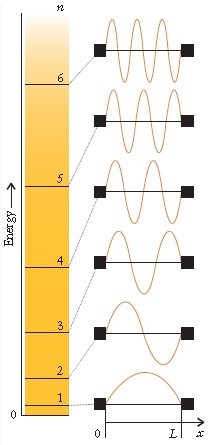
\includegraphics{images/figura1.png}
    \end{figure}

    \par Pela definição clássica da funçaõ de onda $\Psi(\mathbf{x})$, temos:

    \begin{equation}\label{eq_schrodinger_eq2}
        \Psi (\mathbf{x}) = A \cdot sen(k \cdot \mathbf{x}) + B \cdot cos(k \cdot \mathbf{x})
    \end{equation}

    %TODO - QUAIS CONDIÇÕES SÃO ESSAS?
    \par Pela equação de Schrödinger, \eqref{eq_schrodinger_eq2} e das condições de contorno para o problema em questão, é possível concluir:

    \begin{equation}\label{eq_schrodinger_eq3}
      E = \frac{\hbar^2}{8 \pi^2 m} \cdot \frac{n^2\pi^2}{L^2} = \frac{\hbar^2 n^2}{8 m L^2},\ com\ n = 1, 2, ...
    \end{equation}

    \par Como $n \in \mathcal{Z} - \{0\}$, a equação \eqref{eq_schrodinger_eq3} mostra que somente alguns valores para energia são aceitos no confinamento dentro de uma caixa de tamanho L. A partir disso, conclui-se que os níveis de energia de uma partícula confinada são discretos e que a energia pode ser quantizada.

    \par Para definir o operador hamiltoniano utilizado para descrever partículas num cristal, começaremos do cristal perfeito, que descreve de maneira geral as relações entre as partículas nesse sistema. A partir dele, serão feitas aproximações para que se chegue no hamiltoniano do elétron livre.

    \subsubsection{Hamiltoniano de um Cristal Perfeito}

      \par Para definir o operador hamiltoniano utilizado para descrever partículas num cristal, começaremos do cristal perfeito, que descreve de maneira geral as relações entre as partículas nesse sistema. A partir dele, serão feitas aproximações para que se chegue no hamiltoniano do elétron livre. (LIVRO REBECA). 
    
      \par O hamiltoniano do cristal perfeito [YU-CARDONA] é dado por:
      %TODO - REVISAR
      \begin{equation}\label{eq_schrodinger_eq4}
        \mathcal{H} = 
          \sum_{i} \frac{p_{i}^2}{2m_{i}} 
          + \sum_{j} \frac{p_{j}^2}{2m_{j}} 
          + \frac{1}{2} \sum_{j', j} \frac{Z_{j} Z_{j'} e^2}{4\pi\epsilon_{0}\left|R_{j} - R_{j'}\right|}-  \sum_{j, i} \frac{Z_{j} e^2}{4\pi\epsilon_{0}\left|r_{i} - R_{j}\right|} 
          + \frac{1}{2} \sum_{i, i'} \frac{e^2}{4\pi\epsilon_{0}\left|r_{i} - r_{i'}\right|}
      \end{equation}

      \par Na expressão \eqref{eq_schrodinger_eq4}, $\epsilon_{0}$ representa a permissividade no vácuo, $r_{i}$ representa a posição do i-ésimo elétron, $R_{j}$ representa a posição do j-ésimo núcleo, $Z_{j}$ representa o número atômico do núcleo, $p_{i}$ e $p_{j}$ representam o operador momento dos elétrons e o operador momento do núcleo, respectivamente. Além disso, os índices $i'$ e $j'$ são índices não identicos a $i$ e $j$.

      \par Para solucionar o hamiltoniano, leva-se em conta que os elétrons nas camadas totalmente preenchidas estão muito próximos ao núcleo, considerando-os como um pacote. Essa junção de elétrons mais internos com o núcleo atômico forma o que se chama por íon-núcleo.
    
      \par A partir disso, serão aplicadas duas aproximações para facilitar a solução do hamiltoniano. A primeira será a aproximação de Born-Oppenheimer.


      \par Essa aproximação divide os átomos em duas grandes regiões. A primeira região trata o núcleo como uma partícula estática no espaço. Já a segunda região lida somente com as partículas na superfície do sistema.

      \par Aplicando a aproximação de Born-Oppenheimer ao hamiltoniano, pode-se separar os cálculos entre os íons-núcleo e os elétrons na camada de valência. Assim, simplifica-se o hamiltoniano como uma soma de hamiltonianos da relação entre os elétrons de valências, entre os íons-núcleo e entre ambas regiões, da seguinte maneira:

      \begin{equation}\label{eq_schrodinger_eq5}
        \mathcal{H} = 
          \mathcal{H}_{ions} (\mathbf{R}_{j}) 
          + \mathcal{H}_{e}(\mathbf{r}_{i}, \mathbf{R}_{j_{0}})
          + \mathcal{H}_{e-ion}(\mathbf{r}_i, \delta\mathbf{R}_j)
      \end{equation}

      \par Nessa expressão, $\mathcal{H}_{ions}(\mathbf{R}_{j})$ é o hamiltoniano referente às interações entre os íons-núcleo que se movimentam devido aos seus potenciais iônicos; $\mathcal{H}_{e}(\mathbf{r}_{i},\mathbf{R}_{j_{0}})$ é o hamiltoniano referente às interações elétron-elétron, considerando os íons-núcleo estáticos e congelados na posição de equilíbrio $\mathbf{R}_{j_{0}}$; $\mathcal{H}_{e-ion}(\mathbf{r}_{i},\delta\mathbf{R}_{j})$ é o hamiltoniano que descreve a interação elétron-íon, caracterizando a variação na energia eletrônica causada pelo deslocamento $\delta\mathbf{R}_{j}$ dos íons-núcleo em relação ao seu ponto de equilíbrio $\mathbf{R}_{j_{0}}$.
      
      \par Escrevendo o hamiltoniano do cristal perfeito, retirando os termos referentes unicamente ao núcleo e mantendo as interações elétron-elétron, obtém-se:

      \begin{equation}\label{eq_schrodinger_eq6}
        \mathcal{H}_{e} = 
          \sum_{i} \frac{p_{i}^2}{2m_{i}} 
          -  \sum_{j, i} \frac{Z_{j} e^2}{4\pi\epsilon_{0}\left|r_{i} - R_{j_{0}}\right|} 
          + \frac{1}{2} \sum_{i, i'} \frac{e^2}{4\pi\epsilon_{0}\left|r_{i} - r_{i'}\right|}
      \end{equation}

      \par Para simplificar a equação \eqref{eq_schrodinger_eq6}, será utilizada a aproximação mean-field. Essa aproximação consiste na escolha de um local arbitrário para o elétron no sistema e na consideração de que os outros graus de liberdade se encontram estáticos se utilizarmos seu valor médio. Aplicando o hamiltoniano somente em um elétron, tem-se que:

      \begin{equation}\label{eq_schrodinger_eq7}
        \mathcal{H}_{1e} = \frac{p^2}{2m}
      \end{equation}

      Considerando que o operador momento,na mecânica quântica, é definido por:

      \begin{equation}\label{eq_schrodinger_eq8}
        p = -i\hbar\frac{d}{dx} \Longrightarrow
        p^2 = -\hbar^2 \frac{d^2}{dx^2} \Longrightarrow
        p^2 = -\hbar^2 \nabla^2
      \end{equation}

      Aplicando \eqref{eq_schrodinger_eq8} em \eqref{eq_schrodinger_eq7}, tem-se:

      \begin{equation}\label{eq_schrodinger_eq9}
        \mathcal{H}_{1e} = - \frac{\hbar^2}{2m}\nabla^2
      \end{equation}

      Define-se assim, o operador hamiltonia para o caso considerado. Aplicando a equação de Schrödinger ao caso do elétron livre, no qual o potencial U(\textbf{r}) é igual a zero, tem-se que:

      \begin{equation}\label{eq_schrodinger_eq10}
        \mathcal{H} \cdot \Psi(\mathbf{r}) =
          -\frac{\hbar^2}{2m} \nabla^2 \Psi(\mathbf{r}) =
          E \cdot \Psi(\mathbf{r})
      \end{equation}

      Com autovalores de energia dados por:

      \begin{equation}\label{eq_schrodinger_autovalores}
        E = \frac{\hbar^2 k^2}{2m}
      \end{equation}

      Em uma rede cristalina, o elétron sofre influência de um potencial. Esse potencial pode ser tratado como um potencial periódico [ASHCROFT] em alguns casos e será explicado a seguir.

      


      




% Vamos colocar uma equação aqui para deixar as coisas mais interessantes,
% \begin{align}\label{e=mc}
% 	E = mc^2.
% \end{align}
% Podemos nos referenciar a equação \eqref{e=mc}.
 
\subsection{Alguns detalhes}

% Para maiores detalhes sobre como escrever em \LaTeX, vide \cite{lshort}.

\subsubsection{Detalhes ainda mais detalhados}
Clique no link.

\phantomsection
\addcontentsline{toc}{section}{Referências}
\begin{thebibliography}{99}
% INTRODUÇÃO
\bibitem{introducao1} de Figueiredo Oliveira, André Rezende. \href{http://www.infis.ufu.br/sites/infis.ufu.br/files/Anexos/Bookpage/TCC%20F%C3%8DSICA%20DE%20MATERIAIS%202009_2%20-%20ANDRE%20REZENDE.pdf}
\textit{Caracterização Óptica de Pontos Quânticos Semicondutores de CdS em Matrizes Poliméricas}. 
\bibitem{introducao2} Ekimov, Alexey I., and Alexei A. Onushchenko. \href{https://www.researchgate.net/profile/Alexey_Onushchehko/publication/234289541_Quantum_Size_Effect_in_Three-Dimensional_Microscopic_Semiconductor_Crystals/links/0c9605305fa93c4e3d000000.pdf}\textit{Quantum size effect in three-dimensional microscopic semiconductor crystals. Jetp Lett 34.6 (1981): 345-349}.
\bibitem{introducao3} Brus, Louis E. \href{http://aip.scitation.org/doi/10.1063/1.447218}\textit{Electron-electron and electron-hole interactions in small semiconductor crystallites: The size dependence of the lowest excited electronic state. The Journal of chemical physics 80.9 (1984): 4403-4409}.
\bibitem{introducao4} Murray, CBea, David J. Norris, and Moungi G. Bawendi. \href{http://pubs.acs.org/doi/abs/10.1021/ja00072a025?journalCode=jacsat}\textit{Synthesis and characterization of nearly monodisperse CdE (E= sulfur, selenium, tellurium) semiconductor nanocrystallites. Journal of the American Chemical Society 115.19 (1993): 8706-8715}.
\bibitem{introducao5} Zhu, Jun-Jie, et al. \href{https://link.springer.com/book/10.1007/978-3-642-44910-9}\textit{Quantum dots for DNA biosensing. Vol. 165. Springer, 2013}.
% INTRODUÇÃO A MECÂNICA QUÂNTICA E FÍSICA DO ESTADO SÓLIDO
  %Redes Cristalinas
\bibitem{qm_fis1} QM with applications to nanotech and information
\bibitem{qm_fis2} LIVRO REBECCA
  %Equação de Schrödinger
\bibitem{qm_fis3} Eisberg, Robert Martin; Resnick, Robert - \textit{Física Quântica} %TODO - HREF
\bibitem{qm_fis4} C.W. Sherwin- \textit{"Introduction to quantum mechanics" - Holt, Rinehart \& Winston of Canada Ltd (1959)}. %TODO - HREF
% FRUSTRADO
 \bibitem{frustrado1} Eisberg, Robert Martin Resnick, and Cota Araiza Robert. \href{http://gen.lib.rus.ec/book/index.php?md5=80CCC290E6FFF645ADF0BA24178E4C5D}\textit{Física cuántica: átomos, moléculas, sólidos, núcleos y partículas. 1994}.
 \bibitem{frustrado2} Atkins, Peter, and Loretta Jones. \href{http://gen.lib.rus.ec/book/index.php?md5=6D32E94CECA0A9BD6FFF5F1307078071}\textit{Chemical principles: The quest for insight. Macmillan, 2007}.
 \bibitem{frustrado3} Peter, Y. U., and Manuel Cardona. \href{http://gen.lib.rus.ec/book/index.php?md5=20A8507AB491C812ED2C75D08740987A}\textit{Fundamentals of semiconductors: physics and materials properties. Springer Science \& Business Media, 2010}.
 \bibitem{frustrado5} Dagotto, Elbio. \href{http://gen.lib.rus.ec/book/index.php?md5=3C621FEBFE1EBBF8B376CED188D04A84}\textit{Nanoscale phase separation and colossal magnetoresistance: the physics of manganites and related compounds. Vol. 136. Springer Science \& Business Media, 2013}.
 \bibitem{frustrado6} de Lima Rodrigues, Rafael. \href{http://sbfisica.org.br/rbef/pdf/v19_68.pdf}\textit{"Mecânica Quântica na Descrição de Schrödinger." Revista Brasileira de Ensino de Física 19.1 (1997)}.
 \end{thebibliography}
\end{document}
